\documentclass[aspectratio=169,10pt]{beamer}
\usetheme{Madrid}
\usecolortheme{default}
\usepackage{tikz}
\usepackage{booktabs}
\usepackage{fontawesome5}
\usepackage{xcolor}
\usepackage{amsmath}
\usepackage{colortbl}
\usepackage{multirow}
\usetikzlibrary{arrows.meta,shadows,positioning,fit,shapes.geometric,calc}

% ── palette ──────────────────────────────────────────────────────────
\definecolor{c1}{RGB}{41,128,185}
\definecolor{c2}{RGB}{52,152,219}
\definecolor{c3}{RGB}{155,89,182}
\definecolor{c4}{RGB}{142,68,173}
\definecolor{c5}{RGB}{230,126,34}
\definecolor{c6}{RGB}{211,84,0}
\definecolor{hit}{RGB}{39,174,96}
\definecolor{miss}{RGB}{192,57,43}
\definecolor{warn}{RGB}{243,156,18}

\setbeamercolor{frametitle}{bg=c1,fg=white}
\setbeamercolor{title}{fg=white}
\setbeamercolor{structure}{fg=c1}
\setbeamertemplate{navigation symbols}{}
\setbeamertemplate{footline}[frame number]
\setbeamerfont{frametitle}{series=\bfseries}

\newcommand{\chit}[1]{\cellcolor{hit!30} #1}
\newcommand{\cmiss}[1]{\cellcolor{miss!25} #1}
\newcommand{\cwarn}[1]{\cellcolor{warn!30} #1}
\newcommand{\czero}{\cellcolor{black!4} }

\title{\textbf{Graph-Based Vulnerability Retrieval}\\[4pt]}
\subtitle{Master's Thesis — Technical Progress · Checkpoint 5}
\author{Lívia}
\institute{TU Munich · Siemens}
\date{\today}


\begin{document}

% ── title ─────────────────────────────────────────────────────────────
\begin{frame}
\titlepage
\end{frame}

% ── agenda ────────────────────────────────────────────────────────────
\begin{frame}{Agenda}
  \begin{enumerate}
    \item[\textcolor{c1}{\faIcon{redo}}]
      \textbf{Checkpoint 4 recap} — PCA \& L2 ablation results

    \vspace{0.45em}
    \item[\textcolor{c5}{\faIcon{blender}}]
      \textbf{Embedding fusion strategies [Updated results]} — 3-way combination \& 4-way CodeBERT experiment

    
    \vspace{0.45em}
    \item[\textcolor{c3}{\faIcon{microscope}}]
      \textbf{Embedding space analysis updated results} — single-space \& cross-space diagnostics

    \vspace{0.45em}
    \item[\textcolor{c2}{\faIcon{robot}}]
      \textbf{Agent patching: First Variations and Insights} — LLM patch generation by analogy

    \vspace{0.45em}
    \item[\textcolor{c4}{\faIcon{exchange-alt}}]
      \textbf{Prompt variation experiment} — 4 prompt variants on 41-query subset

    \vspace{0.45em}
    \item[\textcolor{hit}{\faIcon{lightbulb}}]
      \textbf{Key findings \& next steps}
  \end{enumerate}
\end{frame}

% ══════════════════════════════════════════════════════════════════════
\section{Recap}
% ══════════════════════════════════════════════════════════════════════

\begin{frame}[fragile]{Checkpoint 4 Recap}
  \centering
  {\Large\textcolor{c1}{Pipeline validation: PCA \& L2 normalization}}

% Combined Embedding Pipeline: Where PCA \& L2 Normalization Sit

  \centering
  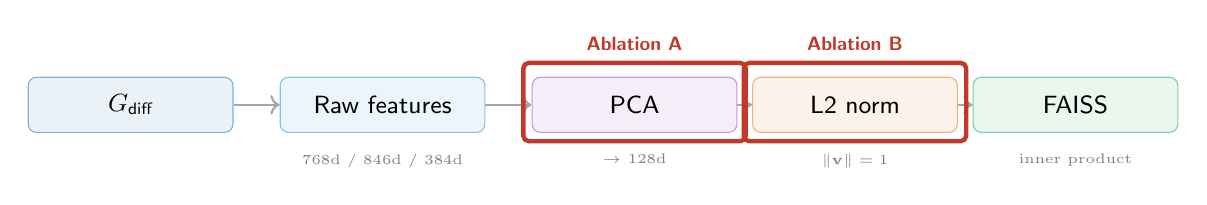
\begin{tikzpicture}[
    box/.style={rounded corners=3pt, draw=#1!60, fill=#1!10,
                minimum width=2.6cm, minimum height=0.7cm,
                font=\small\sffamily, align=center},
    arr/.style={->, thick, gray!70},
    ablbl/.style={font=\scriptsize\sffamily\bfseries, #1}]

    % pipeline boxes
    \node[box=c1]  (graph)  at (0,0)     {$G_{\text{diff}}$};
    \node[box=c2]  (feat)   at (3.2,0)   {Raw features};
    \node[box=c3]  (pca)    at (6.4,0)   {PCA};
    \node[box=c5]  (l2)     at (9.2,0)   {L2 norm};
    \node[box=hit] (faiss)  at (12.0,0)  {FAISS};

    \draw[arr] (graph) -- (feat);
    \draw[arr] (feat)  -- (pca);
    \draw[arr] (pca)   -- (l2);
    \draw[arr] (l2)    -- (faiss);

    % dimension annotations
    \node[below=4pt, font=\tiny\color{black!50}] at (feat.south) {768d / 846d / 384d};
    \node[below=4pt, font=\tiny\color{black!50}] at (pca.south) {$\to$ 128d};
    \node[below=4pt, font=\tiny\color{black!50}] at (l2.south) {$\|\mathbf{v}\|=1$};
    \node[below=4pt, font=\tiny\color{black!50}] at (faiss.south) {inner product};

    % ablation markers
    \draw[miss, ultra thick, rounded corners=2pt]
      ([shift={(-3pt,5pt)}]pca.north west) rectangle ([shift={(3pt,-3pt)}]pca.south east);
    \node[ablbl=miss, above=6pt] at (pca.north) {Ablation A};

    \draw[miss, ultra thick, rounded corners=2pt]
      ([shift={(-3pt,5pt)}]l2.north west) rectangle ([shift={(3pt,-3pt)}]l2.south east);
    \node[ablbl=miss, above=6pt] at (l2.north) {Ablation B};
  \end{tikzpicture}

\end{frame}

% ══════════════════════════════════════════════════════════════════════
\section{Embedding Fusion Strategies}
% ══════════════════════════════════════════════════════════════════════

\begin{frame}[fragile]{Combination Strategies: Experiment Design}
\begin{columns}[T]
\begin{column}{0.50\textwidth}

  \textbf{Goal}\\[3pt]
  {\small The Combined embedder concatenates NetLSD~$+$~WL~$+$~GIN
  then reduces with PCA\@.  Does pre-processing each sub-embedder
  \emph{before} concatenation improve the fused space?}

  

  % \vspace{0.4em}
  % \textbf{Rationale}\\[2pt]
  % {\scriptsize Individual PCA or normalization could equalize sub-embedder
  % scales and remove noise before fusion.  Alternatively, a single
  % final PCA may better exploit cross-embedder correlations.}

\end{column}
\begin{column}{0.47\textwidth}
  \textbf{Strategies compared}
  \vspace{0.2em}

  {\scriptsize
  \begin{tabular}{p{2.2cm}p{4.4cm}}
    \toprule
    \textbf{Strategy} & \textbf{Pipeline} \\
    \midrule
    \texttt{concat\_pca}
      & Concatenate raw $\to$ PCA to 128d {\small(baseline)} \\
    \texttt{pca\_concat\_pca}
      & PCA each to 128d $\to$ concat (384d) $\to$ PCA to 128d \\
    \texttt{pca\_concat}
      & PCA each to 42d $\to$ concat to 126d {\small(no 2\textsuperscript{nd} PCA)} \\
    \texttt{norm\_concat\_pca}
      & L2-norm each $\to$ concat $\to$ PCA to 128d \\
    \bottomrule
  \end{tabular}}
  
\end{column}
\end{columns}
\end{frame}


\begin{frame}{Combination Strategies: Updated Results ($n{=}73$)}

  \centering
  \vspace{0.2em}
  {\small
  \renewcommand{\arraystretch}{1.35}
  \setlength{\tabcolsep}{4.5pt}
  \begin{tabular}{l *{6}{c} }
    \toprule
    & \multicolumn{6}{c}{\textbf{Retrieval}} \\
    \cmidrule{2-7} 
    \textbf{Strategy}
      & hit@1 & hit@5 & hit@10 & MRR & nDCG@10 & MAP@10 \\
    \midrule
    \rowcolor{c1!7}
    \texttt{norm\_concat\_pca}
      & \chit{80.8\%} & \chit{93.2\%} & \chit{95.9\%} & \chit{.849} & \chit{.645} & \chit{.514} \\
    \texttt{concat\_pca}
      & \cmiss{64.4\%} & \cmiss{79.5\%} & \cmiss{84.9\%} & \cmiss{.707} & \cmiss{.452} & \cmiss{.336} \\
    \texttt{pca\_concat\_pca}
      & \cmiss{64.4\%} & \cmiss{79.5\%} & \cmiss{84.9\%} & \cmiss{.707} & \cmiss{.452} & \cmiss{.336} \\
    \texttt{pca\_concat}
      & \cmiss{64.4\%} & \cmiss{78.1\%} & \cmiss{83.6\%} & \cmiss{.706} & \cmiss{.449} & \cmiss{.334} \\
    \addlinespace[3pt]
    \multicolumn{7}{l}{\scriptsize\textit{4-way fusion (+ CodeBERT-pattern)}} \\
    \addlinespace[1pt]
    \texttt{4way\_concat\_pca}
      & \cmiss{64.4\%} & \cmiss{79.5\%} & \cmiss{84.9\%} & \cmiss{.707} & \cmiss{.452} & \cmiss{.336} \\
    \texttt{4way\_norm\_concat\_pca}
      & \cwarn{72.6\%} & \cwarn{86.3\%} & \cwarn{87.7\%} & \cwarn{.773} & \cwarn{.569} & \cwarn{.440} \\
    \bottomrule
  \end{tabular}}

\end{frame}

\begin{frame}[fragile]{4-Way Fusion: Pipeline Comparison}

  \centering
  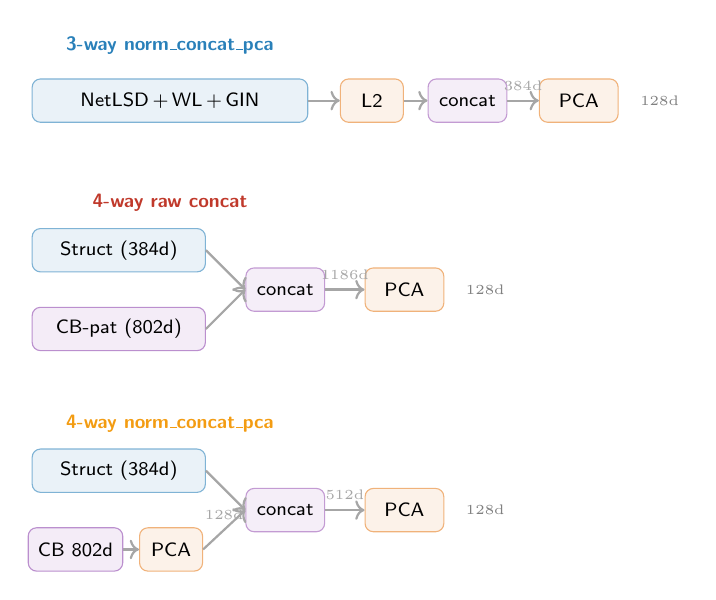
\begin{tikzpicture}[
    box/.style={rounded corners=3pt, draw=#1!60, fill=#1!10,
                minimum height=0.55cm, font=\scriptsize\sffamily, align=center},
    arr/.style={->, thick, gray!70},
    node distance=0.3cm]

    % 3-way baseline
    \node[font=\scriptsize\sffamily\bfseries,c1] (lbl3) at (0,3.0) {3-way norm\_concat\_pca};
    \node[box=c1, minimum width=3.5cm] (c3) at (0,2.3) {NetLSD\,+\,WL\,+\,GIN};
    \node[box=c5, right=0.4cm of c3, minimum width=0.8cm] (l23) {L2};
    \node[box=c3, right=0.3cm of l23, minimum width=1cm] (cat3) {concat};
    \node[box=c5, right=0.4cm of cat3, minimum width=1cm] (pca3) {PCA};
    \draw[arr] (c3) -- (l23);
    \draw[arr] (l23) -- (cat3);
    \draw[arr] (cat3) -- node[above,font=\tiny] {384d} (pca3);
    \node[right=0.15cm of pca3, font=\tiny\color{black!50}] {128d};

    % 4-way run 1: raw concat (no norm)
    \node[font=\scriptsize\sffamily\bfseries,miss] (lbl4a) at (0,1.0) {4-way raw concat};
    \node[box=c1, minimum width=2.2cm] (s4a) at (-0.65,0.4) {Struct (384d)};
    \node[box=c4, minimum width=2.2cm] (cb4a) at (-0.65,-0.6) {CB-pat (802d)};
    \node[box=c3, right=0.5cm of s4a, minimum width=1cm, yshift=-0.5cm] (cat4a) {concat};
    \node[box=c5, right=0.5cm of cat4a, minimum width=1cm] (pca4a) {PCA};
    \draw[arr] (s4a.east) -- (cat4a.west);
    \draw[arr] (cb4a.east) -- (cat4a.west);
    \draw[arr] (cat4a) -- node[above,font=\tiny] {1186d} (pca4a);
    \node[right=0.15cm of pca4a, font=\tiny\color{black!50}] {128d};

    % 4-way run 2: norm_concat_pca
    \node[font=\scriptsize\sffamily\bfseries,warn] (lbl4b) at (0,-1.8) {4-way norm\_concat\_pca};
    \node[box=c1, minimum width=2.2cm] (s4b) at (-0.65,-2.4) {Struct (384d)};
    \node[box=c4, minimum width=1.2cm] (cb4b) at (-1.2,-3.4) {CB 802d};
    \node[box=c5, right=0.2cm of cb4b, minimum width=0.8cm] (pcb) {\scriptsize PCA};
    \node[box=c3, right=0.5cm of s4b, minimum width=1cm, yshift=-0.5cm] (cat4b) {concat};
    \node[box=c5, right=0.5cm of cat4b, minimum width=1cm] (pca4b) {PCA};
    \draw[arr] (s4b.east) -- (cat4b.west);
    \draw[arr] (cb4b) -- (pcb);
    \draw[arr] (pcb.east) -- node[above,font=\tiny] {128d} (cat4b.west);
    \draw[arr] (cat4b) -- node[above,font=\tiny] {512d} (pca4b);
    \node[right=0.15cm of pca4b, font=\tiny\color{black!50}] {128d};
  \end{tikzpicture}

\end{frame}


\begin{frame}{Visualizing the Embedding Space: Methodology}
\begin{columns}[T]
\begin{column}{0.50\textwidth}

  \textbf{Goal}\\[3pt]
  {\small Understand how different embedding strategies structure the
  vulnerability space and whether PCA preserves neighbourhood quality.}

  \vspace{0.6em}
  \textbf{Embedders compared}
  \begin{itemize}\setlength{\itemsep}{3pt}
    \item \textbf{CodeBERT-pattern} --- CodeBERT applied to extracted
          code \textit{patterns} from the diff graph (802d raw: 34d pattern $+$ 768d CodeBERT)
    \item \textbf{Combined} --- NetLSD~$+$~WL~$+$~GIN structural
          embedders concatenated (384d raw)
  \end{itemize}

\end{column}
\begin{column}{0.47\textwidth}

  \textbf{Visualization pipeline}

  \vspace{0.3em}
  {\scriptsize
  \begin{enumerate}\setlength{\itemsep}{3pt}
    \item Extract embeddings for all CVE variants
    \item For each embedder, produce two views:
      \begin{itemize}\setlength{\itemsep}{1pt}
        \item \textbf{Raw} (high-dim, L2-normed) $\to$ t-SNE to 2D
        \item \textbf{PCA$\to$128d + L2} $\to$ t-SNE to 2D
      \end{itemize}
    \item Color points by \textbf{CWE class}; mark query samples
          with black open circles
  \end{enumerate}}

  \vspace{0.5em}
  {\scriptsize\textcolor{c1}{\faIcon{info-circle}}
  Side-by-side comparison reveals whether PCA dimensionality
  reduction preserves or improves CWE cluster structure.}

\end{column}
\end{columns}
\end{frame}
\begin{frame}{Space Analysis}
\begin{figure}
  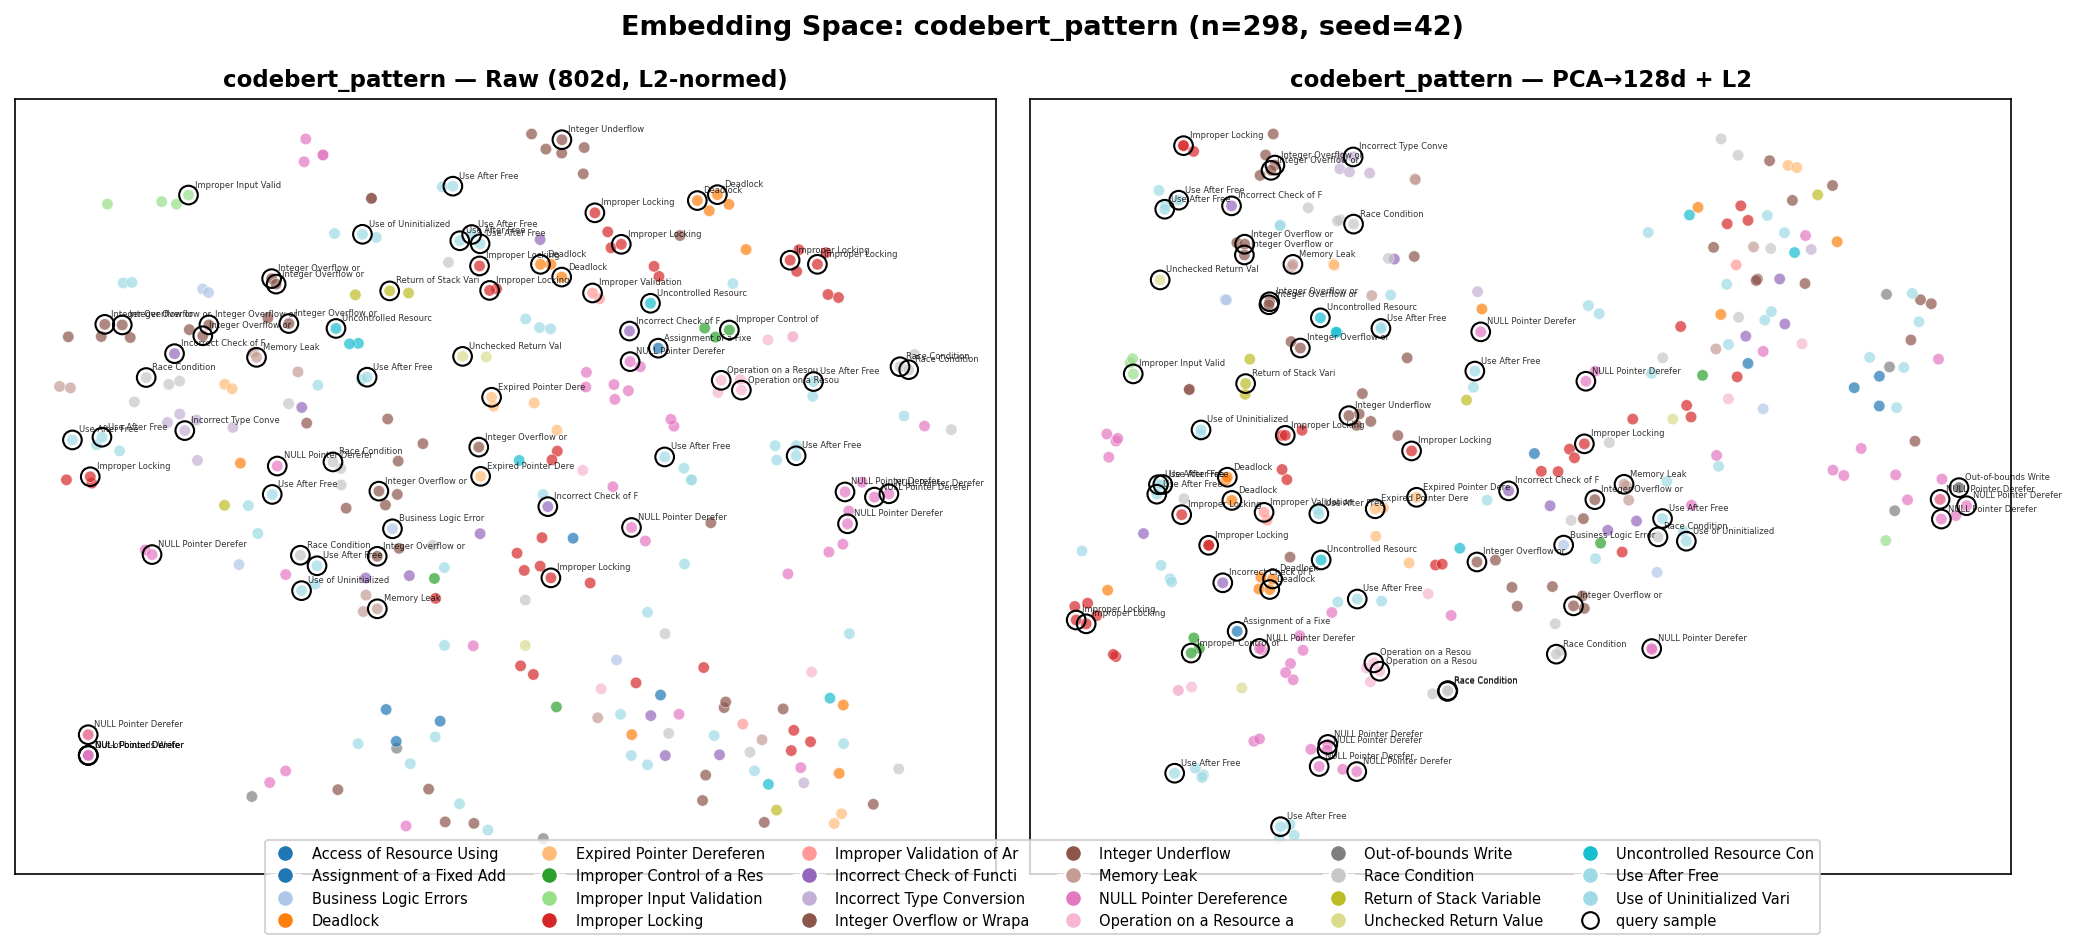
\includegraphics[width=\linewidth]{../../experiments/output/checkpoint5/plots/embedding_spaces/codebert_pattern_raw_vs_pca.png}
\end{figure}
\end{frame}

\begin{frame}{Space Analysis}
  \begin{figure}
    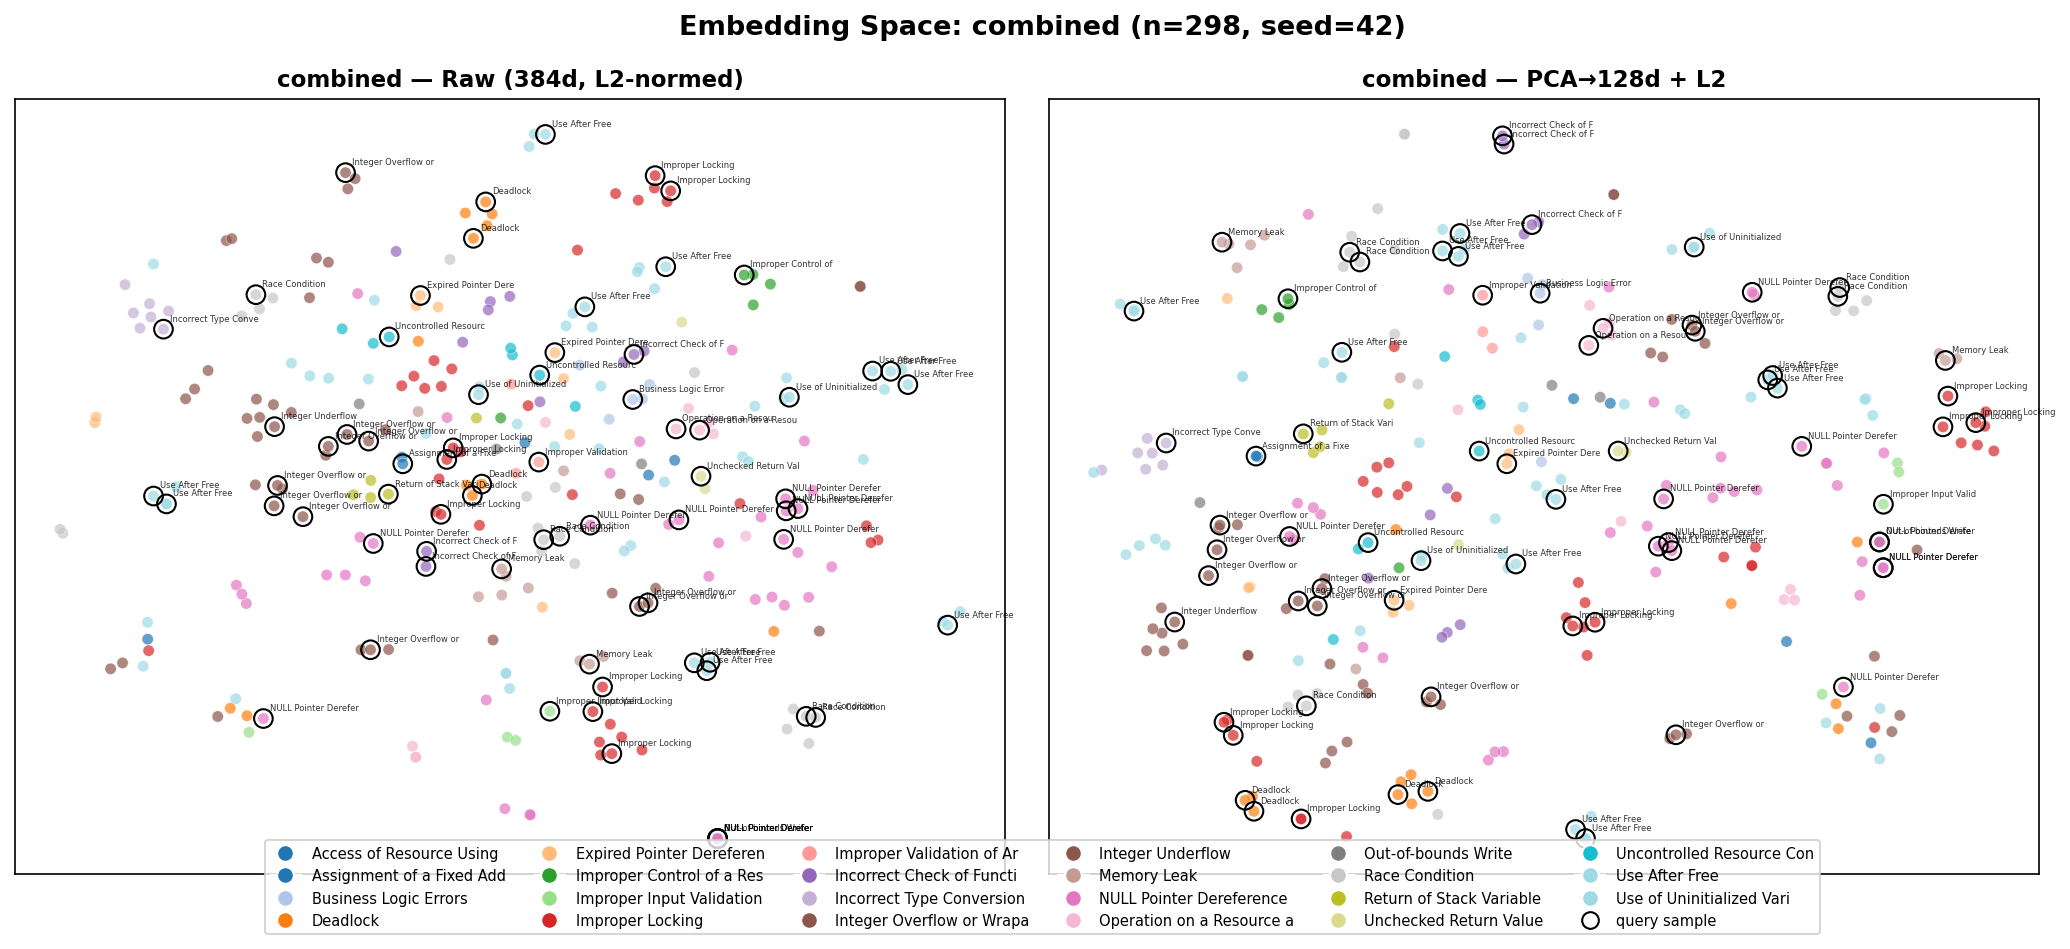
\includegraphics[width=\linewidth]{../../experiments/output/checkpoint5/plots/embedding_spaces/combined_raw_vs_pca.png}
  \end{figure}

\end{frame}

\begin{frame}{Space Analysis: Interpretation}

  \begin{columns}[T]
  \begin{column}{0.48\textwidth}

    \textbf{\textcolor{c1}{CodeBERT-pattern (802d $\to$ 128d)}}

    \vspace{0.3em}
    {\small
    \begin{itemize}\setlength{\itemsep}{3pt}
      \item[\textcolor{hit}{\faIcon{check-circle}}]
        Distinct clusters for NULL Pointer Dereference
        and Uncontrolled Resource Consumption ---
        CodeBERT captures code-level vulnerability semantics

      \item[\textcolor{miss}{\faIcon{times-circle}}]
        Central region is ``muddy'': Business Logic Errors
        and Improper Input Validation overlap, indicating
        these CWEs share similar code patterns

      \item[\textcolor{c1}{\faIcon{crosshairs}}]
        Query samples (black circles) land on top of
        same-class index samples --- good k-NN retrieval
        despite cluttered global structure
    \end{itemize}}

  \end{column}
  \begin{column}{0.48\textwidth}

    \textbf{\textcolor{c3}{Combined vs.\ CodeBERT-pattern}}

    \vspace{0.3em}
    {\small
    \begin{itemize}\setlength{\itemsep}{3pt}
      \item[\textcolor{c3}{\faIcon{project-diagram}}]
        CodeBERT-pattern produces tighter CWE clusters;
        Combined (structural) is more blended ---
        code-semantic features separate vulnerability
        types more clearly than graph-structural features

      \item[\textcolor{c5}{\faIcon{compress-arrows-alt}}]
        PCA (802d $\to$ 128d) preserves cluster structure
        in CodeBERT-pattern with 99.4\% variance explained,
        confirming the raw space is largely low-rank

      \item[\textcolor{c1}{\faIcon{chart-bar}}]
        Despite better visual clustering, CodeBERT-pattern
        retrieval (hit@1$=$71.2\%) trails Combined
        (hit@1$=$89.0\%) --- local neighbourhood quality
        matters more than global separation
    \end{itemize}}

  \end{column}
  \end{columns}

\end{frame}

\begin{frame}[fragile]{GIN Training: Experiment Design}
\begin{columns}[T]
\begin{column}{0.50\textwidth}

  \textbf{Goal}\\[3pt]
  {\small Can we improve the frozen GIN embedder (random weights,
  seed-42) by fine-tuning with \textbf{triplet metric learning}?
  Compare two feature strategies: structural vs.\ CodeBERT.}
  % TODO: check a reference for the network architecture
  \vspace{0.5em}
  \textbf{Shared architecture}\\[2pt]
  {\scriptsize
  \texttt{input\_proj $\to$ 3$\times$GINConv(MLP) + BatchNorm}\\
  \texttt{$\to$ add\_pool $\Vert$ mean\_pool $\to$ readout $\to$ L2}\\[3pt]
  Output: 128d L2-normalized.\\
  Loss: \texttt{TripletMarginLoss(p=2)}, semi-hard mining every 5 epochs.\\
  Optimizer: Adam, weight decay $10^{-4}$, gradient clip 1.0.}

\end{column}
\begin{column}{0.47\textwidth}

  \textbf{Two variants}

  \vspace{0.2em}
  {\scriptsize
  \renewcommand{\arraystretch}{1.2}
  \setlength{\tabcolsep}{2.5pt}
  \begin{tabular}{l p{2.8cm} p{2.8cm}}
    \toprule
    & \textbf{GIN-Struct} & \textbf{GIN-CodeBERT} \\
    \midrule
    Node feat.
      & 11d one-hot (AST type)
      & 768d CodeBERT per node \\
    Init
      & \textbf{Warm start} from frozen GIN weights
      & Random init \\
    Triplet labels
      & CVE-ID (64 classes)
      & CWE-ID (23 classes) \\
    Margin
      & 0.5 & 0.3 \\
    LR / sched.
      & 5$\times 10^{-4}$ / cosine
      & $10^{-3}$ / constant \\
    Dropout
      & 0.2 & 0.3 \\
    \bottomrule
  \end{tabular}}

  \vspace{0.4em}
  {\scriptsize\textcolor{c1}{\faIcon{info-circle}}
  \textbf{Warm start}: copy frozen GIN's exact parameters,
  then fine-tune --- preserves known-good structural geometry.}

\end{column}
\end{columns}
\end{frame}


\begin{frame}{GIN Training: Results}

  \centering
  \vspace{0.2em}
  {\small
  \renewcommand{\arraystretch}{1.35}
  \setlength{\tabcolsep}{5pt}
  \begin{tabular}{l c c c c c c c}
    \toprule
    \textbf{Model}
      & \textbf{Epochs}
      & \textbf{Train loss}
      & \textbf{hit@1}
      & \textbf{hit@10}
      & \textbf{MRR}
      & \textbf{CWE recall}
      & \textbf{CVE F1} \\
    \midrule
    Frozen GIN (baseline)
      & --- & --- & 72.6\% & 90.4\% & .788 & .443 & --- \\
    \rowcolor{hit!10}
    \textbf{GIN-Struct} (trained)
      & 94 & \chit{.012} & \chit{78.1\%} & \chit{94.5\%} & \chit{.826} & \chit{.578} & \chit{.808} \\
    \rowcolor{miss!10}
    GIN-CodeBERT (trained)
      & 42 & \cmiss{.151} & \cmiss{28.8\%} & \cmiss{57.5\%} & \cmiss{.372} & \cmiss{.212} & \cmiss{.296} \\
    \addlinespace[3pt]
    \multicolumn{8}{l}{\scriptsize\textit{Reference (untrained combined embedders)}} \\
    \addlinespace[1pt]
    Combined (N+WL+GIN)
      & --- & --- & 89.0\% & 97.3\% & .916 & .498 & --- \\
    \bottomrule
  \end{tabular}}

  \vspace{0.6em}
  \begin{columns}[T]
    \begin{column}{0.48\textwidth}
      {\scriptsize\textbf{\textcolor{hit}{GIN-Struct: strong}}}\\[2pt]
      {\scriptsize
      \begin{itemize}\setlength{\itemsep}{2pt}
        \item Warm start $+$ CVE-level triplets $\to$ hit@1 improves
              72.6\% $\to$ 78.1\% (+5.5pp)
        \item CWE recall jumps 44.3\% $\to$ 57.8\% ---
              better cross-class generalization
        \item Approaches Combined (89\%) using a \textit{single}
              embedder with only 11d node features
      \end{itemize}}
    \end{column}
    \begin{column}{0.48\textwidth}
      {\scriptsize\textbf{\textcolor{miss}{GIN-CodeBERT: failed}}}\\[2pt]
      {\scriptsize
      \begin{itemize}\setlength{\itemsep}{2pt}
        \item 768d CodeBERT node features did not help ---
              hit@1 drops to 28.8\%, worse than frozen GIN
        \item Loss plateaus at 0.151 (vs.\ 0.012 for Struct),
              model does not converge
        \item CWE-level labels too coarse for CVE-level retrieval;
              random init loses structural geometry
      \end{itemize}}
    \end{column}
  \end{columns}
\end{frame}

\begin{frame}
  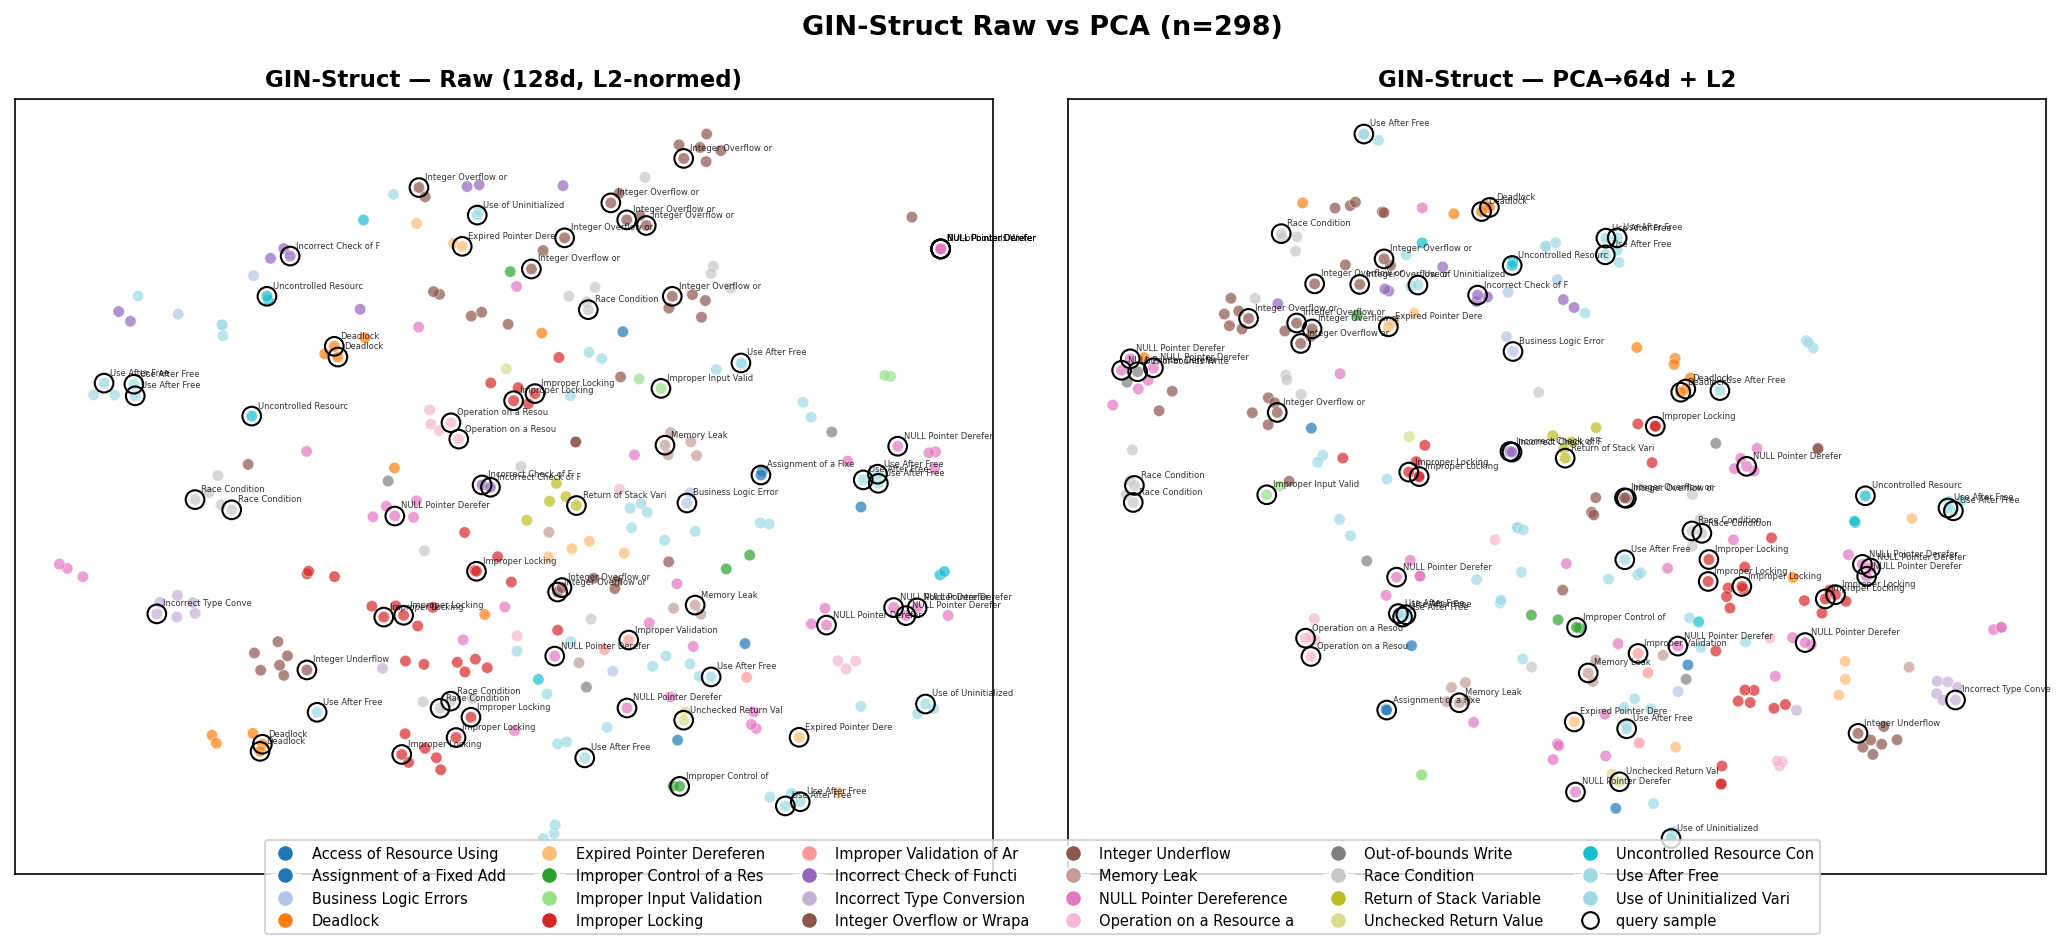
\includegraphics[width=\textwidth]{../../experiments/output/checkpoint5/gin_struct_raw_vs_pca.png}
\end{frame}
% ══════════════════════════════════════════════════════════════════════
\section{Agent Baseline}
% ══════════════════════════════════════════════════════════════════════

\begin{frame}{[RECAP] Agent Baseline: Experiment Design}
\begin{columns}[T]
\begin{column}{0.52\textwidth}

  \textbf{Goal}\\[3pt]
  {\small Given a vulnerable function and a retrieved similar CVE,
  can an LLM generate a correct patch \textbf{by analogy}?
  Compare \textit{oracle} retrieval (perfect) vs.\ \textit{embedding} retrieval (our pipeline).}

  \vspace{0.6em}
  \textbf{Model \& prompt}
  \begin{itemize}\setlength{\itemsep}{2pt}
    {\scriptsize
    \item \textbf{GPT-4o} (Azure), temperature$=$0.2, max\_tokens$=$4096
    \item \textbf{One-shot patching by analogy}: system prompt contains the
          retrieved CVE's fix-list, variable/function mapping, root cause
    \item Assistant message shows the example's CoT + patched code
    \item User message provides the target function to patch
    \item Agent must output \texttt{[CoT START]...[Patched Code END]}}
  \end{itemize}

\end{column}
\end{columns}
\end{frame}


\begin{frame}{[RECAP] Agent Baseline: Per-CWE Oracle vs.\ Embedding (BERTScore \& ROUGE-L)}

  \centering
  \vspace{-0.2em}
  {\tiny
  \renewcommand{\arraystretch}{1.15}
  \setlength{\tabcolsep}{2.5pt}
  \begin{tabular}{l r c c c c c c c}
    \toprule
    \textbf{CWE class}
      & \textbf{n}
      & \textbf{hit@1 (\%)}
      & \textbf{Orac.\ BERT}
      & \textbf{Emb.\ BERT}
      & \textbf{$\Delta$\%}
      & \textbf{Orac.\ RG-L}
      & \textbf{Emb.\ RG-L}
      & \textbf{$\Delta$\%} \\
    \midrule
    \rowcolor{hit!8}
    Fixed Address to Pointer          & 1  & \chit{100}  & .969 & .969 & 0.0            & .993 & .993 & 0.0 \\
    Resource Lifetime                 & 1  & \chit{100}  & .934 & .934 & 0.0            & .951 & .951 & 0.0 \\
    Memory Leak                       & 2  & \chit{100}  & .911 & .902 & $-$0.9         & .926 & .921 & $-$0.6 \\
    Check Return Value                & 3  & \cwarn{33}  & .904 & .603 & \cmiss{$-$33.3}& .934 & .613 & \cmiss{$-$34.4} \\
    Use After Free                    & 12 & \cwarn{75}  & .861 & .721 & \cmiss{$-$16.2}& .874 & .748 & \cmiss{$-$14.4} \\
    Uninitialized Variable            & 2  & \chit{100}  & .841 & .853 & \chit{+1.4}   & .953 & .961 & \chit{+0.8} \\
    Return of Stack Var               & 1  & \chit{100}  & .815 & .820 & +0.6           & .883 & .864 & $-$2.1 \\
    Type Conversion                   & 1  & \chit{100}  & .802 & .692 & \cmiss{$-$13.6}& .978 & .978 & 0.0 \\
    \midrule
    Deadlock                          & 4  & \chit{100}  & .767 & .726 & $-$5.4         & .833 & .842 & +1.1 \\
    Resource Expiration               & 2  & \cwarn{50}  & .765 & .725 & $-$5.3         & .854 & .838 & $-$1.8 \\
    Array Index Validation            & 1  & \cmiss{0}   & .720 & .882 & \chit{+22.6}  & .745 & .959 & \chit{+28.7} \\
    Input Validation                  & 1  & \cmiss{0}   & .715 & .715 & 0.0            & .689 & .689 & 0.0 \\
    Race Condition                    & 5  & \chit{100}  & .703 & .712 & \chit{+1.2}   & .689 & .731 & \chit{+6.1} \\
    Integer Overflow                  & 10 & \cwarn{60}  & .699 & .705 & \chit{+0.9}   & .829 & .804 & $-$3.1 \\
    Business Logic                    & 1  & \chit{100}  & .689 & .750 & \chit{+8.9}   & .702 & .769 & \chit{+9.6} \\
    Integer Underflow                 & 1  & \chit{100}  & .681 & .726 & \chit{+6.6}   & .840 & .880 & \chit{+4.7} \\
    \midrule
    NULL Pointer Deref                & 11 & \cmiss{36}  & .629 & .683 & \chit{+8.6}   & .710 & .723 & +1.8 \\
    Expired Pointer Deref             & 2  & \chit{100}  & .587 & .583 & $-$0.8         & .466 & .468 & +0.5 \\
    Improper Locking                  & 8  & \chit{100}  & .565 & .550 & $-$2.6         & .544 & .525 & $-$3.4 \\
    Resource Exhaustion               & 2  & \cmiss{0}   & .539 & .710 & \chit{+31.7}  & .649 & .665 & \chit{+2.4} \\
    Unchecked Return Value            & 1  & \cmiss{0}   & .428 & .495 & \chit{+15.6}  & .466 & .603 & \chit{+29.4} \\
    Out-of-bounds Write               & 1  & \cmiss{0}   & .151 & .008 & \cmiss{$-$94.6}& .454 & .670 & \chit{+47.6} \\
    \midrule
    \rowcolor{c1!8}
    \textbf{Overall}                  & \textbf{73} & \textbf{68.5}
                                      & \textbf{.716} & \textbf{.691} & \textbf{$-$3.5}
                                      & \textbf{.766} & \textbf{.741} & \textbf{$-$3.3} \\
    \bottomrule
  \end{tabular}}

  \vspace{0.3em}
  {\scriptsize
  \textcolor{c1}{\faIcon{info-circle}} hit@1 = \% queries where FAISS top-1 matches the correct CVE.
  \textcolor{hit}{\faIcon{check-circle}} 12/22 CWEs: embedding $\ge$ oracle \quad
  \textcolor{miss}{\faIcon{times-circle}} Low hit@1 does \textbf{not} always mean low BERT/RG-L (e.g.\ Array Index, Resource Exhaustion)}

\end{frame}


% ══════════════════════════════════════════════════════════════════════
\section{LLM Semantic Evaluation}
% ══════════════════════════════════════════════════════════════════════

\begin{frame}{[RECAP] LLM Semantic Evaluation: Experiment Design}
\begin{columns}[T]
\begin{column}{0.50\textwidth}

  \textbf{Goal}\\[3pt]
  {\small Text-similarity metrics (BLEU, Jaccard) measure \textit{surface overlap}
  with the ground truth, not whether the vulnerability is actually fixed.
  Can an LLM judge the \textbf{semantic correctness} of a patch?}

  \vspace{0.6em}
  \textbf{Rationale}\\[3pt]
  {\small A patch can be textually different yet semantically correct
  (e.g.\ different variable names, reordered guards).
  Conversely, a high-BLEU patch may miss the critical fix.
  We need a \textbf{vulnerability-aware} evaluation.}

  \vspace{0.6em}
  \textbf{Scope}\\[3pt]
  {\small All 73 oracle-mode patches from the agent baseline, evaluated
  with GPT-4o as a security auditor.}

\end{column}
\begin{column}{0.47\textwidth}

  \textbf{Prompt design}

  \vspace{0.3em}
  {\scriptsize
  \begin{enumerate}\setlength{\itemsep}{3pt}
    \item \textbf{Role:} ``Expert security code auditor specializing
          in vulnerability analysis''
    \item \textbf{Input:} CVE ID, CWE class, vulnerability description,
          original vulnerable code, generated patch
    \item \textbf{Task:} Determine if the patch fixes the specific
          vulnerability described
    \item \textbf{Output format:} structured JSON with
          \texttt{verdict} (FIXED / NOT\_FIXED / PARTIAL),
          \texttt{confidence} (0.0--1.0),
          \texttt{reasoning} (free text)
  \end{enumerate}}

  \vspace{0.5em}
  \textbf{Model \& parameters}
  {\scriptsize
  \begin{itemize}\setlength{\itemsep}{2pt}
    \item \textbf{GPT-4o} (Azure), temperature$=$0
    \item Deterministic evaluation (no sampling variance)
    \item 1.5s delay between calls (rate limiting)
  \end{itemize}}

\end{column}
\end{columns}
\end{frame}


\begin{frame}{[RECAP] LLM Semantic Evaluation: Preliminary Results ($n{=}73$)}

  \begin{columns}[T]
  \begin{column}{0.45\textwidth}

  \centering
  \vspace{0.5em}
  {\small
  \renewcommand{\arraystretch}{1.35}
  \setlength{\tabcolsep}{5pt}
  \begin{tabular}{l c c}
    \toprule
    \textbf{Verdict} & \textbf{Count} & \textbf{\%} \\
    \midrule
    \rowcolor{hit!12}
    FIXED       & 41 & 56.2\% \\
    \rowcolor{warn!12}
    PARTIAL     &  4 &  5.5\% \\
    \rowcolor{miss!12}
    NOT\_FIXED  & 28 & 38.4\% \\
    \midrule
    \rowcolor{c1!8}
    \textbf{Fix rate} (FIXED $+$ PARTIAL) & \textbf{45} & \textbf{61.6\%} \\
    \bottomrule
  \end{tabular}}

  \vspace{0.8em}
  {\scriptsize
  \renewcommand{\arraystretch}{1.25}
  \begin{tabular}{l c}
    \toprule
    \textbf{Verdict} & \textbf{Avg.\ confidence} \\
    \midrule
    FIXED       & 0.948 \\
    NOT\_FIXED  & 0.902 \\
    PARTIAL     & 0.750 \\
    \midrule
    \textbf{Overall} & \textbf{0.919} \\
    \bottomrule
  \end{tabular}}

  \end{column}
  \begin{column}{0.52\textwidth}

  \centering
  \vspace{0.5em}
  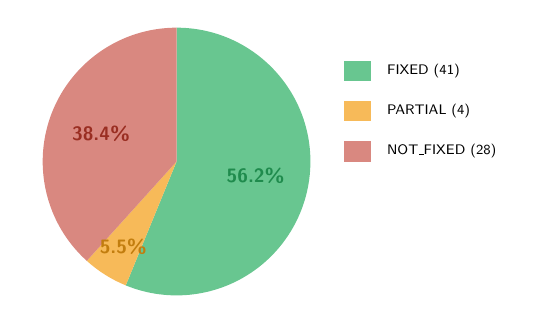
\begin{tikzpicture}[scale=0.85]
    % Pie chart
    \def\radius{2}
    % FIXED: 56.2% -> 202.3 degrees
    \fill[hit!70] (0,0) -- (90:\radius) arc (90:-112.3:\radius) -- cycle;
    % PARTIAL: 5.5% -> 19.8 degrees
    \fill[warn!70] (0,0) -- (-112.3:\radius) arc (-112.3:-132.1:\radius) -- cycle;
    % NOT_FIXED: 38.4% -> 138.2 degrees
    \fill[miss!60] (0,0) -- (-132.1:\radius) arc (-132.1:-270:\radius) -- cycle;

    \node[font=\scriptsize\sffamily\bfseries,hit!80!black] at (350:\radius*0.6) {56.2\%};
    \node[font=\scriptsize\sffamily\bfseries,warn!80!black] at (238:\radius*0.75) {5.5\%};
    \node[font=\scriptsize\sffamily\bfseries,miss!80!black] at (160:\radius*0.6) {38.4\%};

    % Legend
    \fill[hit!70] (2.5,1.2) rectangle (2.9,1.5);
    \node[right,font=\tiny\sffamily] at (3.0,1.35) {FIXED (41)};
    \fill[warn!70] (2.5,0.6) rectangle (2.9,0.9);
    \node[right,font=\tiny\sffamily] at (3.0,0.75) {PARTIAL (4)};
    \fill[miss!60] (2.5,0.0) rectangle (2.9,0.3);
    \node[right,font=\tiny\sffamily] at (3.0,0.15) {NOT\_FIXED (28)};
  \end{tikzpicture}

  \vspace{0.6em}
  {\scriptsize\color{black!55}
  Model: GPT-4o (Azure), temperature$=$0.\\
  Run: \texttt{python -m src.evaluate.llm\_evaluation results.jsonl}}

  \end{column}
  \end{columns}
\end{frame}


\begin{frame}{[RECAP] LLM Semantic Evaluation: Per-CWE Breakdown}

  \centering
  \vspace{-0.4em}
  {\tiny
  \renewcommand{\arraystretch}{1.15}
  \setlength{\tabcolsep}{3pt}
  \begin{tabular}{l r c c c c c}
    \toprule
    \textbf{CWE class}
      & \textbf{n}
      & \textbf{hit@1 CVE (\%)}
      & \textbf{FIXED}
      & \textbf{PARTIAL}
      & \textbf{NOT\_FIXED}
      & \textbf{Fix rate} \\
    \midrule
    \rowcolor{hit!8}
    Array Index Validation     & 1  & \cmiss{0}   & 1 & 0 & 0 & \chit{100\%} \\
    \rowcolor{hit!8}
    Business Logic             & 1  & \chit{100}  & 1 & 0 & 0 & \chit{100\%} \\
    \rowcolor{hit!8}
    Input Validation           & 1  & \cmiss{0}   & 1 & 0 & 0 & \chit{100\%} \\
    \rowcolor{hit!8}
    Integer Underflow          & 1  & \chit{100}  & 1 & 0 & 0 & \chit{100\%} \\
    \rowcolor{hit!8}
    Out-of-bounds Write        & 1  & \cmiss{0}   & 1 & 0 & 0 & \chit{100\%} \\
    \rowcolor{hit!8}
    Resource Expiration        & 2  & \cwarn{50}  & 2 & 0 & 0 & \chit{100\%} \\
    \rowcolor{hit!8}
    Unchecked Return Value     & 1  & \cmiss{0}   & 1 & 0 & 0 & \chit{100\%} \\
    \rowcolor{hit!8}
    Uninitialized Variable     & 2  & \chit{100}  & 2 & 0 & 0 & \chit{100\%} \\
    \addlinespace[2pt]
    Integer Overflow           & 10 & \cwarn{60}  & 7 & 2 & 1 & \chit{90.0\%} \\
    Use After Free             & 12 & \cwarn{75}  & 10 & 0 & 2 & \chit{83.3\%} \\
    Race Condition             & 5  & \chit{100}  & 3 & 0 & 2 & 60.0\% \\
    Deadlock                   & 4  & \chit{100}  & 2 & 0 & 2 & 50.0\% \\
    Improper Locking           & 8  & \chit{100}  & 3 & 1 & 4 & 50.0\% \\
    Memory Leak                & 2  & \chit{100}  & 1 & 0 & 1 & 50.0\% \\
    Resource Exhaustion        & 2  & \cmiss{0}   & 1 & 0 & 1 & 50.0\% \\
    \addlinespace[2pt]
    \rowcolor{miss!8}
    NULL Pointer Deref         & 11 & \cmiss{36}  & 3 & 1 & 7 & \cmiss{36.4\%} \\
    \rowcolor{miss!8}
    Check Return Value         & 3  & \cwarn{33}  & 1 & 0 & 2 & \cmiss{33.3\%} \\
    \rowcolor{miss!8}
    Expired Pointer Deref      & 2  & \chit{100}  & 0 & 0 & 2 & \cmiss{0\%} \\
    \rowcolor{miss!8}
    Fixed Address to Pointer   & 1  & \chit{100}  & 0 & 0 & 1 & \cmiss{0\%} \\
    \rowcolor{miss!8}
    Resource Lifetime          & 1  & \chit{100}  & 0 & 0 & 1 & \cmiss{0\%} \\
    \rowcolor{miss!8}
    Return of Stack Var        & 1  & \chit{100}  & 0 & 0 & 1 & \cmiss{0\%} \\
    \rowcolor{miss!8}
    Type Conversion            & 1  & \chit{100}  & 0 & 0 & 1 & \cmiss{0\%} \\
    \midrule
    \rowcolor{c1!8}
    \textbf{Overall}           & \textbf{73} & \textbf{68.5} & \textbf{41} & \textbf{4} & \textbf{28} & \textbf{61.6\%} \\
    \bottomrule
  \end{tabular}}

\end{frame}
% ══════════════════════════════════════════════════════════════════════
\section{Prompt Variation Experiment}
% ══════════════════════════════════════════════════════════════════════

% ── Slide 1: Experiment Design ────────────────────────────────────────
\begin{frame}{Prompt Variation: Experiment Design}
  \begin{columns}[T]
    \begin{column}{0.52\textwidth}
      \textbf{\textcolor{c1}{Goal}}\\[3pt]
      Measure how the agent's system prompt affects patch quality.
      Four variants alter CoT depth and whether graph context is
      injected into the target slot.

      \vspace{0.6em}
      \textbf{\textcolor{c3}{Setup}}\\[3pt]
      \begin{itemize}\setlength{\itemsep}{2pt}
        \item Same 41-query subset (39 unique CVE/variant pairs)
        \item Oracle retrieval, GPT-4o, temperature$=$0.2
        \item Metrics: BLEU-4, BERTScore F1, ROUGE-L, Jaccard, LLM fix rate
      \end{itemize}
    \end{column}
    \begin{column}{0.45\textwidth}
      {\scriptsize
      \renewcommand{\arraystretch}{1.2}
      \setlength{\tabcolsep}{2.5pt}
      \begin{tabular}{l p{4.0cm}}
        \toprule
        \textbf{Variant} & \textbf{Key difference} \\
        \midrule
        \texttt{default}
          & 3-step CoT (describe $\to$ generate $\to$ output) \\
        \texttt{graph}
          & 6-step CoT + CPG analysis + graph context in target \\
        \texttt{graph\_v2}
          & Verification step + patch diff as graph context \\
        \texttt{default\_v2}
          & 3-step CoT + explicit root-cause confirmation \\
        \bottomrule
      \end{tabular}}
    \end{column}
  \end{columns}
\end{frame}

% ── Slide 1b: Pipeline Schemas ────────────────────────────────────────
\begin{frame}[fragile]{Prompt Variation: Pipeline Comparison}
  \centering
  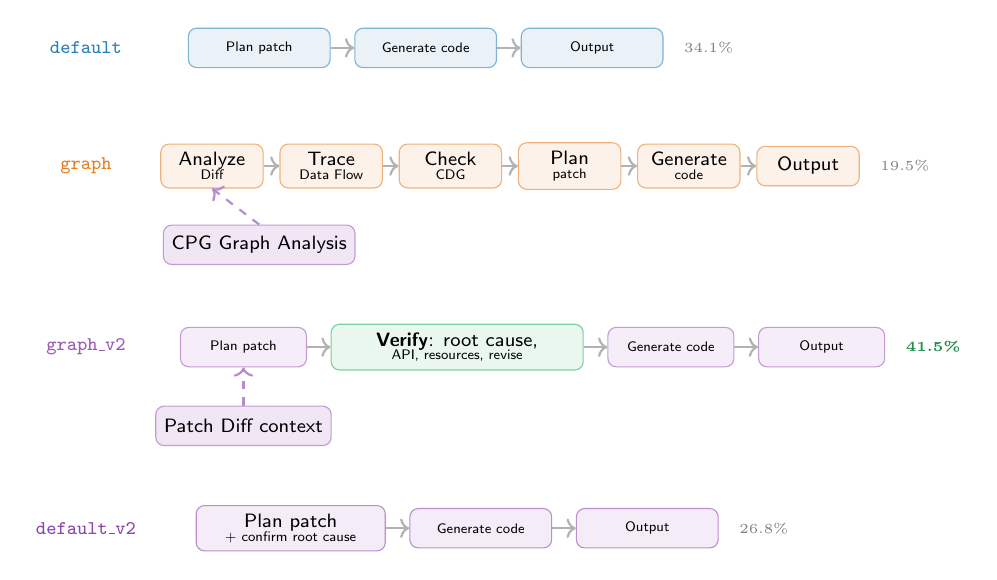
\begin{tikzpicture}[
    box/.style={rounded corners=3pt, draw=#1!60, fill=#1!10,
                minimum height=0.5cm, font=\tiny\sffamily, align=center},
    lbl/.style={font=\scriptsize\sffamily\bfseries, #1},
    arr/.style={->, thick, gray!60},
    garr/.style={->, thick, c3!70, dashed},
    node distance=0.25cm and 0.25cm,
    every node/.style={inner sep=3pt}]

    % ── default ──────────────────────────────────────────────
    \node[lbl=c1] (ld) at (-6.2, 3.3) {\texttt{default}};
    \node[box=c1, minimum width=1.8cm] (d1) at (-4.0, 3.3) {Plan patch};
    \node[box=c1, minimum width=1.8cm, right=0.3cm of d1] (d2) {Generate code};
    \node[box=c1, minimum width=1.8cm, right=0.3cm of d2] (d3) {Output};
    \draw[arr] (d1) -- (d2);
    \draw[arr] (d2) -- (d3);
    \node[right=0.15cm of d3, font=\tiny\color{black!50}] {34.1\%};

    % ── graph ────────────────────────────────────────────────
    \node[lbl=c5] (lg) at (-6.2, 1.8) {\texttt{graph}};
    \node[box=c5, minimum width=1.3cm] (g1) at (-4.6, 1.8) {\scriptsize Analyze\\[-1pt]Diff};
    \node[box=c5, minimum width=1.3cm, right=0.2cm of g1] (g2) {\scriptsize Trace\\[-1pt]Data Flow};
    \node[box=c5, minimum width=1.3cm, right=0.2cm of g2] (g3) {\scriptsize Check\\[-1pt]CDG};
    \node[box=c5, minimum width=1.3cm, right=0.2cm of g3] (g4) {\scriptsize Plan\\[-1pt]patch};
    \node[box=c5, minimum width=1.3cm, right=0.2cm of g4] (g5) {\scriptsize Generate\\[-1pt]code};
    \node[box=c5, minimum width=1.3cm, right=0.2cm of g5] (g6) {\scriptsize Output};
    \draw[arr] (g1) -- (g2);
    \draw[arr] (g2) -- (g3);
    \draw[arr] (g3) -- (g4);
    \draw[arr] (g4) -- (g5);
    \draw[arr] (g5) -- (g6);
    % graph context annotation
    \node[box=c3, minimum width=2.4cm, fill=c3!15] (gc) at (-4.0, 0.8) {\scriptsize CPG Graph Analysis};
    \draw[garr] (gc.north) -- (g1.south);
    \node[right=0.15cm of g6, font=\tiny\color{black!50}] {19.5\%};

    % ── graph_v2 ─────────────────────────────────────────────
    \node[lbl=c3] (lgv) at (-6.2, -0.5) {\texttt{graph\_v2}};
    \node[box=c3, minimum width=1.6cm] (v1) at (-4.2, -0.5) {Plan patch};
    \node[box=hit, minimum width=3.2cm, right=0.3cm of v1] (v2)
      {\scriptsize \textbf{Verify}: root cause,\\[-1pt]API, resources, revise};
    \node[box=c3, minimum width=1.6cm, right=0.3cm of v2] (v3) {Generate code};
    \node[box=c3, minimum width=1.6cm, right=0.3cm of v3] (v4) {Output};
    \draw[arr] (v1) -- (v2);
    \draw[arr] (v2) -- (v3);
    \draw[arr] (v3) -- (v4);
    % patch diff annotation
    \node[box=c3, minimum width=2.0cm, fill=c3!15] (pd) at (-4.2, -1.5) {\scriptsize Patch Diff context};
    \draw[garr] (pd.north) -- (v1.south);
    \node[right=0.15cm of v4, font=\tiny\color{hit!80!black}] {\textbf{41.5\%}};

    % ── default_v2 ───────────────────────────────────────────
    \node[lbl=c4] (ldv) at (-6.2, -2.8) {\texttt{default\_v2}};
    \node[box=c4, minimum width=2.4cm] (dv1) at (-3.6, -2.8)
      {\scriptsize Plan patch\\[-1pt]{\tiny+ confirm root cause}};
    \node[box=c4, minimum width=1.8cm, right=0.3cm of dv1] (dv2) {Generate code};
    \node[box=c4, minimum width=1.8cm, right=0.3cm of dv2] (dv3) {Output};
    \draw[arr] (dv1) -- (dv2);
    \draw[arr] (dv2) -- (dv3);
    \node[right=0.15cm of dv3, font=\tiny\color{black!50}] {26.8\%};

  \end{tikzpicture}

  \vspace{0.3em}
  {\scriptsize
  \textcolor{c3}{\faIcon{project-diagram}} Dashed arrows = graph context injection \qquad
  \textcolor{hit}{\faIcon{shield-alt}} Green box = explicit verification step \qquad
  Percentages = LLM fix rate}
\end{frame}

% ── Slide 1c: Key Differences Summary ────────────────────────────────
\begin{frame}{Prompt Variation: Key Differences Summary}
  \centering
  \vspace{0.3em}
  {\small
  \renewcommand{\arraystretch}{1.4}
  \setlength{\tabcolsep}{4pt}
  \begin{tabular}{l c c c c}
    \toprule
    \textbf{Aspect}
      & \texttt{\textbf{default}}
      & \texttt{\textbf{graph}}
      & \texttt{\textbf{graph\_v2}}
      & \texttt{\textbf{default\_v2}} \\
    \midrule
    CoT steps
      & 3 & 6 & 4 & 3 \\
    CPG data in prompt
      & \textcolor{miss}{\faIcon{times}} None
      & \textcolor{hit}{\faIcon{check}} Full
      & \textcolor{c5}{\faIcon{minus}} Diff only
      & \textcolor{miss}{\faIcon{times}} None \\
    Verification checklist
      & \textcolor{miss}{\faIcon{times}}
      & \textcolor{miss}{\faIcon{times}}
      & \textcolor{hit}{\faIcon{check}}
      & \textcolor{miss}{\faIcon{times}} \\
    Root-cause confirmation
      & \textcolor{miss}{\faIcon{times}}
      & \textcolor{miss}{\faIcon{times}}
      & \textcolor{hit}{\faIcon{check}} {\tiny(in verify)}
      & \textcolor{hit}{\faIcon{check}} {\tiny(1 sentence)} \\
    Assistant shows verification
      & \textcolor{miss}{\faIcon{times}}
      & \textcolor{miss}{\faIcon{times}}
      & \textcolor{hit}{\faIcon{check}}
      & \textcolor{miss}{\faIcon{times}} \\
    \midrule
    \rowcolor{c1!8}
    \textbf{LLM fix rate}
      & 34.1\%
      & \cmiss{19.5\%}
      & \chit{41.5\%}
      & 26.8\% \\
    \bottomrule
  \end{tabular}}

  \vspace{0.6em}
  {\scriptsize
  \textcolor{c1}{\faIcon{info-circle}}
  \textbf{Full CPG} = Patch Diff + Data Flow + Control Dependencies \qquad
  \textbf{Diff only} = Patch Diff section (lines changed, AST types)}
\end{frame}

% ── Slide 2: Results Comparison ───────────────────────────────────────
\begin{frame}{Prompt Variation: Results ($n{=}41$)}
  \centering
  \vspace{-0.3em}
  {\scriptsize
  \renewcommand{\arraystretch}{1.35}
  \setlength{\tabcolsep}{5pt}
  \begin{tabular}{l c c c c c}
    \toprule
    \textbf{Variant}
      & \textbf{BLEU-4}
      & \textbf{BERTScore F1}
      & \textbf{ROUGE-L}
      & \textbf{Tok.\ Jaccard}
      & \textbf{LLM Fix Rate} \\
    \midrule
    \texttt{default}
      & .652 & .718 & .752 & .724
      & 34.1\% {\tiny(14/41)} \\
    \texttt{graph}
      & .638 & \chit{.728} & .746 & .718
      & 19.5\% {\tiny(8/41)} \\
    \rowcolor{c3!12}
    \texttt{graph\_v2}
      & \chit{.654} & .723 & \chit{.753} & \chit{.722}
      & \chit{41.5\%} {\tiny(17/41)} \\
    \texttt{default\_v2}
      & .638 & .716 & .740 & .716
      & 26.8\% {\tiny(11/41)} \\
    \bottomrule
  \end{tabular}}

  \vspace{0.5em}
  \begin{columns}[T]
    \begin{column}{0.32\textwidth}
      {\scriptsize\textbf{\textcolor{c1}{Text metrics}}}\\[2pt]
      {\scriptsize
      \begin{itemize}\setlength{\itemsep}{1pt}
        \item All variants within 2.5\% of each other
        \item \texttt{graph\_v2} and \texttt{default} lead
      \end{itemize}}
    \end{column}
    \begin{column}{0.32\textwidth}
      {\scriptsize\textbf{\textcolor{c3}{LLM fix rate}}}\\[2pt]
      {\scriptsize
      \begin{itemize}\setlength{\itemsep}{1pt}
        \item \texttt{graph\_v2} leads at 41.5\%
        \item \texttt{graph} drops to 19.5\%
      \end{itemize}}
    \end{column}
    \begin{column}{0.32\textwidth}
      {\scriptsize\textbf{\textcolor{c5}{Divergence}}}\\[2pt]
      {\scriptsize
      \begin{itemize}\setlength{\itemsep}{1pt}
        \item Text similarity $\neq$ semantic fix
        \item Verification step matters most
      \end{itemize}}
    \end{column}
  \end{columns}
\end{frame}

% ── Slide 3: Analysis ────────────────────────────────────────────────
\begin{frame}{Prompt Variation: Analysis}
  \begin{enumerate}\setlength{\itemsep}{0.3em}

    \item[\textcolor{hit}{\faIcon{check-circle}}]
      \textbf{Verification step is the strongest lever.}
      \texttt{graph\_v2} adds ``VERIFY root cause, API compliance,
      resource ownership'' and reaches 41.5\% fix rate ---
      2$\times$ the base \texttt{graph} variant (19.5\%).

    \item[\textcolor{miss}{\faIcon{times-circle}}]
      \textbf{Raw graph context hurts without structure.}
      \texttt{graph} injects CPG analysis but achieves the lowest
      fix rate (19.5\%), suggesting unstructured graph data
      distracts the model from the fix pattern.

    \item[\textcolor{c3}{\faIcon{chart-bar}}]
      \textbf{Text metrics are near-indistinguishable.}
      $\Delta$BLEU-4 across all variants is only 0.016 (2.5\%).
      LLM-as-judge reveals quality differences invisible
      to surface-level n-gram overlap.

    \item[\textcolor{c5}{\faIcon{lightbulb}}]
      \textbf{Root-cause confirmation alone is insufficient.}
      \texttt{default\_v2} adds ``confirm your plan addresses
      root cause'' but only reaches 26.8\% --- the verification
      checklist in \texttt{graph\_v2} is more actionable.

  \end{enumerate}
\end{frame}


% ══════════════════════════════════════════════════════════════════════
\section{Key Findings \& Next Steps}
% ══════════════════════════════════════════════════════════════════════

\begin{frame}{Key Findings}

  \begin{enumerate}\setlength{\itemsep}{0.5em}
    \item[\textcolor{c1}{\faIcon{search}}]
      \textbf{Retrieval hit@1: 89.0\% overall, but varies by CWE.}
      12/22 CWEs have perfect retrieval; 8/22 have hit@1 $\le$ 75\%.
      Some CWEs (e.g.\ Resource Exhaustion) have low hit@1 but high
      BERT/RG-L, suggesting the embedding retrieves semantically
      relevant analogies even if not the exact CVE.

    \vspace{0.3em}
    \item[\textcolor{c3}{\faIcon{robot}}]
      \textbf{Embedding retrieval nearly matches oracle for patching.}
      Oracle BLEU .655 / Embedding .637 ($-$2.7\%); ROUGE-L .766 / .741 ($-$3.3\%).
      Stereotyped CWEs (Use After Free, Integer Overflow) patch well;
      complex locking refactors remain hard (.34).

    \vspace{0.3em}
    \item[\textcolor{c4}{\faIcon{shield-alt}}]
      \textbf{LLM semantic evaluation: 61.6\% of patches fix the CVE.}
      GPT-4o as security auditor confirms 41/73 fully fixed $+$ 4 partial.
      Retrieval$\to$generation gap (89\%$\to$62\%) shows
      the bottleneck is fix transfer, not analogy retrieval.

    \vspace{0.3em}
    \item[\textcolor{c3}{\faIcon{exchange-alt}}]
      \textbf{Verification prompts double fix rate vs.\ raw graph context.}
      \texttt{graph\_v2} (41.5\%) vs.\ \texttt{graph} (19.5\%) on the
      same 41 queries (the hardest). Text metrics are near-identical ($\Delta$BLEU~2.5\%);
      LLM-as-judge exposes the real quality gap.

  \end{enumerate}
\end{frame}


\begin{frame}{Next Steps}

  \begin{enumerate}\setlength{\itemsep}{0.5em}

    \item[\textcolor{c1}{\faIcon{search}}]
      \textbf{Analyse retrieval failure modes.}
      Embedding loses 14--16\% on Use After Free --- investigate
      which CVE variants are mis-retrieved and whether reranking helps.

  \end{enumerate}
\end{frame}


\begin{frame}[plain]
\centering
\vspace{3em}
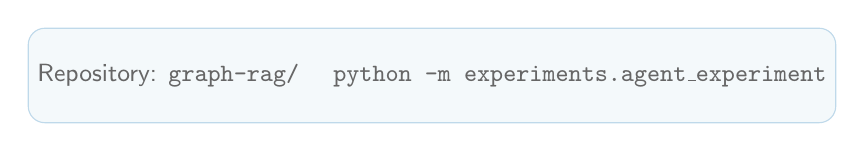
\begin{tikzpicture}
  \node[draw=c1!30,rounded corners=6pt,fill=c1!5,
        minimum width=9cm,minimum height=1.2cm,
        font=\small\sffamily\color{black!60},align=center]
    {Repository: \texttt{graph-rag/} \quad
     \texttt{python -m experiments.agent\_experiment}};
\end{tikzpicture}
\end{frame}

\end{document}
